\documentclass{ximera}

%\usepackage{todonotes}

\newcommand{\todo}{}

\usepackage{esint} % for \oiint
\ifxake%%https://math.meta.stackexchange.com/questions/9973/how-do-you-render-a-closed-surface-double-integral
\renewcommand{\oiint}{{\large\bigcirc}\kern-1.56em\iint}
\fi


\graphicspath{
  {./}
  {ximeraTutorial/}
  {basicPhilosophy/}
  {functionsOfSeveralVariables/}
  {normalVectors/}
  {lagrangeMultipliers/}
  {vectorFields/}
  {greensTheorem/}
  {shapeOfThingsToCome/}
  {dotProducts/}
  {partialDerivativesAndTheGradientVector/}
  {../productAndQuotientRules/exercises/}
  {../normalVectors/exercisesParametricPlots/}
  {../continuityOfFunctionsOfSeveralVariables/exercises/}
  {../partialDerivativesAndTheGradientVector/exercises/}
  {../directionalDerivativeAndChainRule/exercises/}
  {../commonCoordinates/exercisesCylindricalCoordinates/}
  {../commonCoordinates/exercisesSphericalCoordinates/}
  {../greensTheorem/exercisesCurlAndLineIntegrals/}
  {../greensTheorem/exercisesDivergenceAndLineIntegrals/}
  {../shapeOfThingsToCome/exercisesDivergenceTheorem/}
  {../greensTheorem/}
  {../shapeOfThingsToCome/}
  {../separableDifferentialEquations/exercises/}
  {vectorFields/}
}

\newcommand{\mooculus}{\textsf{\textbf{MOOC}\textnormal{\textsf{ULUS}}}}

\usepackage{tkz-euclide}
\usepackage{tikz}
\usepackage{tikz-cd}
\usetikzlibrary{arrows}
\tikzset{>=stealth,commutative diagrams/.cd,
  arrow style=tikz,diagrams={>=stealth}} %% cool arrow head
\tikzset{shorten <>/.style={ shorten >=#1, shorten <=#1 } } %% allows shorter vectors

\usetikzlibrary{backgrounds} %% for boxes around graphs
\usetikzlibrary{shapes,positioning}  %% Clouds and stars
\usetikzlibrary{matrix} %% for matrix
\usepgfplotslibrary{polar} %% for polar plots
\usepgfplotslibrary{fillbetween} %% to shade area between curves in TikZ
%\usetkzobj{all}
\usepackage[makeroom]{cancel} %% for strike outs
%\usepackage{mathtools} %% for pretty underbrace % Breaks Ximera
%\usepackage{multicol}
\usepackage{pgffor} %% required for integral for loops



%% http://tex.stackexchange.com/questions/66490/drawing-a-tikz-arc-specifying-the-center
%% Draws beach ball
\tikzset{pics/carc/.style args={#1:#2:#3}{code={\draw[pic actions] (#1:#3) arc(#1:#2:#3);}}}



\usepackage{array}
\setlength{\extrarowheight}{+.1cm}
\newdimen\digitwidth
\settowidth\digitwidth{9}
\def\divrule#1#2{
\noalign{\moveright#1\digitwidth
\vbox{\hrule width#2\digitwidth}}}




% \newcommand{\RR}{\mathbb R}
% \newcommand{\R}{\mathbb R}
% \newcommand{\N}{\mathbb N}
% \newcommand{\Z}{\mathbb Z}

\newcommand{\sagemath}{\textsf{SageMath}}


%\renewcommand{\d}{\,d\!}
%\renewcommand{\d}{\mathop{}\!d}
%\newcommand{\dd}[2][]{\frac{\d #1}{\d #2}}
%\newcommand{\pp}[2][]{\frac{\partial #1}{\partial #2}}
% \renewcommand{\l}{\ell}
%\newcommand{\ddx}{\frac{d}{\d x}}

% \newcommand{\zeroOverZero}{\ensuremath{\boldsymbol{\tfrac{0}{0}}}}
%\newcommand{\inftyOverInfty}{\ensuremath{\boldsymbol{\tfrac{\infty}{\infty}}}}
%\newcommand{\zeroOverInfty}{\ensuremath{\boldsymbol{\tfrac{0}{\infty}}}}
%\newcommand{\zeroTimesInfty}{\ensuremath{\small\boldsymbol{0\cdot \infty}}}
%\newcommand{\inftyMinusInfty}{\ensuremath{\small\boldsymbol{\infty - \infty}}}
%\newcommand{\oneToInfty}{\ensuremath{\boldsymbol{1^\infty}}}
%\newcommand{\zeroToZero}{\ensuremath{\boldsymbol{0^0}}}
%\newcommand{\inftyToZero}{\ensuremath{\boldsymbol{\infty^0}}}



% \newcommand{\numOverZero}{\ensuremath{\boldsymbol{\tfrac{\#}{0}}}}
% \newcommand{\dfn}{\textbf}
% \newcommand{\unit}{\,\mathrm}
% \newcommand{\unit}{\mathop{}\!\mathrm}
% \newcommand{\eval}[1]{\bigg[ #1 \bigg]}
% \newcommand{\seq}[1]{\left( #1 \right)}
% \renewcommand{\epsilon}{\varepsilon}
% \renewcommand{\phi}{\varphi}


% \renewcommand{\iff}{\Leftrightarrow}

% \DeclareMathOperator{\arccot}{arccot}
% \DeclareMathOperator{\arcsec}{arcsec}
% \DeclareMathOperator{\arccsc}{arccsc}
% \DeclareMathOperator{\si}{Si}
% \DeclareMathOperator{\scal}{scal}
% \DeclareMathOperator{\sign}{sign}


%% \newcommand{\tightoverset}[2]{% for arrow vec
%%   \mathop{#2}\limits^{\vbox to -.5ex{\kern-0.75ex\hbox{$#1$}\vss}}}
% \newcommand{\arrowvec}[1]{{\overset{\rightharpoonup}{#1}}}
% \renewcommand{\vec}[1]{\arrowvec{\mathbf{#1}}}
% \renewcommand{\vec}[1]{{\overset{\boldsymbol{\rightharpoonup}}{\mathbf{#1}}}}

% \newcommand{\point}[1]{\left(#1\right)} %this allows \vector{ to be changed to \vector{ with a quick find and replace
% \newcommand{\pt}[1]{\mathbf{#1}} %this allows \vec{ to be changed to \vec{ with a quick find and replace
% \newcommand{\Lim}[2]{\lim_{\point{#1} \to \point{#2}}} %Bart, I changed this to point since I want to use it.  It runs through both of the exercise and exerciseE files in limits section, which is why it was in each document to start with.

% \DeclareMathOperator{\proj}{\mathbf{proj}}
% \newcommand{\veci}{{\boldsymbol{\hat{\imath}}}}
% \newcommand{\vecj}{{\boldsymbol{\hat{\jmath}}}}
% \newcommand{\veck}{{\boldsymbol{\hat{k}}}}
% \newcommand{\vecl}{\vec{\boldsymbol{\l}}}
% \newcommand{\uvec}[1]{\mathbf{\hat{#1}}}
% \newcommand{\utan}{\mathbf{\hat{t}}}
% \newcommand{\unormal}{\mathbf{\hat{n}}}
% \newcommand{\ubinormal}{\mathbf{\hat{b}}}

% \newcommand{\dotp}{\bullet}
% \newcommand{\cross}{\boldsymbol\times}
% \newcommand{\grad}{\boldsymbol\nabla}
% \newcommand{\divergence}{\grad\dotp}
% \newcommand{\curl}{\grad\cross}
%\DeclareMathOperator{\divergence}{divergence}
%\DeclareMathOperator{\curl}[1]{\grad\cross #1}
% \newcommand{\lto}{\mathop{\longrightarrow\,}\limits}

% \renewcommand{\bar}{\overline}

\colorlet{textColor}{black}
\colorlet{background}{white}
\colorlet{penColor}{blue!50!black} % Color of a curve in a plot
\colorlet{penColor2}{red!50!black}% Color of a curve in a plot
\colorlet{penColor3}{red!50!blue} % Color of a curve in a plot
\colorlet{penColor4}{green!50!black} % Color of a curve in a plot
\colorlet{penColor5}{orange!80!black} % Color of a curve in a plot
\colorlet{penColor6}{yellow!70!black} % Color of a curve in a plot
\colorlet{fill1}{penColor!20} % Color of fill in a plot
\colorlet{fill2}{penColor2!20} % Color of fill in a plot
\colorlet{fillp}{fill1} % Color of positive area
\colorlet{filln}{penColor2!20} % Color of negative area
\colorlet{fill3}{penColor3!20} % Fill
\colorlet{fill4}{penColor4!20} % Fill
\colorlet{fill5}{penColor5!20} % Fill
\colorlet{gridColor}{gray!50} % Color of grid in a plot

\newcommand{\surfaceColor}{violet}
\newcommand{\surfaceColorTwo}{redyellow}
\newcommand{\sliceColor}{greenyellow}




\pgfmathdeclarefunction{gauss}{2}{% gives gaussian
  \pgfmathparse{1/(#2*sqrt(2*pi))*exp(-((x-#1)^2)/(2*#2^2))}%
}


%%%%%%%%%%%%%
%% Vectors
%%%%%%%%%%%%%

%% Simple horiz vectors
\renewcommand{\vector}[1]{\left\langle #1\right\rangle}


%% %% Complex Horiz Vectors with angle brackets
%% \makeatletter
%% \renewcommand{\vector}[2][ , ]{\left\langle%
%%   \def\nextitem{\def\nextitem{#1}}%
%%   \@for \el:=#2\do{\nextitem\el}\right\rangle%
%% }
%% \makeatother

%% %% Vertical Vectors
%% \def\vector#1{\begin{bmatrix}\vecListA#1,,\end{bmatrix}}
%% \def\vecListA#1,{\if,#1,\else #1\cr \expandafter \vecListA \fi}

%%%%%%%%%%%%%
%% End of vectors
%%%%%%%%%%%%%

%\newcommand{\fullwidth}{}
%\newcommand{\normalwidth}{}



%% makes a snazzy t-chart for evaluating functions
%\newenvironment{tchart}{\rowcolors{2}{}{background!90!textColor}\array}{\endarray}

%%This is to help with formatting on future title pages.
\newenvironment{sectionOutcomes}{}{}



%% Flowchart stuff
%\tikzstyle{startstop} = [rectangle, rounded corners, minimum width=3cm, minimum height=1cm,text centered, draw=black]
%\tikzstyle{question} = [rectangle, minimum width=3cm, minimum height=1cm, text centered, draw=black]
%\tikzstyle{decision} = [trapezium, trapezium left angle=70, trapezium right angle=110, minimum width=3cm, minimum height=1cm, text centered, draw=black]
%\tikzstyle{question} = [rectangle, rounded corners, minimum width=3cm, minimum height=1cm,text centered, draw=black]
%\tikzstyle{process} = [rectangle, minimum width=3cm, minimum height=1cm, text centered, draw=black]
%\tikzstyle{decision} = [trapezium, trapezium left angle=70, trapezium right angle=110, minimum width=3cm, minimum height=1cm, text centered, draw=black]


\title{ArcSine \& ArcCosine}

\begin{document}

\begin{abstract}
restricting the domain
\end{abstract}
\maketitle



To complete the picture on our family of Trigonometric functions, we need some inverse functions.  Since none of our Trigonometric functions are one-to-one functions, we will restrict their domains for the purposes of obtaining inverse functions.





\section*{Arcsine}


The sine function is not one-to-one.









\begin{image}
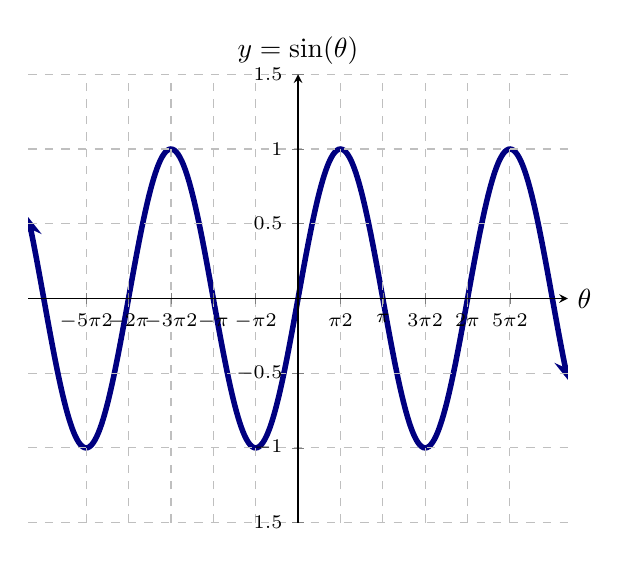
\begin{tikzpicture}
  \begin{axis}[
            domain=-10:10, ymax=1.5, xmax=10, ymin=-1.5, xmin=-10,
            axis lines =center, xlabel={$\theta$}, ylabel={$y = \sin(\theta)$}, grid = major, grid style={dashed},
            ytick={-1.5,-1,-0.5,0.5,1,1.5},
            xtick={-7.85, -6.28, -4.71, -3.14, -1.57, 0, 1.57, 3.142, 4.71, 6.28, 7.85},
            xticklabels={$-\tfrac{5\pi}{2}$,$-2\pi$,$-\tfrac{3\pi}{2}$,$-\pi$, $-\tfrac{\pi}{2}$, $0$, $\tfrac{\pi}{2}$, $\pi$, $\tfrac{3\pi}{2}$, $2\pi$, $\tfrac{5\pi}{2}$},
            yticklabels={$1.5$,$-1$,$-0.5$,$0.5$,$1$,$1.5$}, 
            ticklabel style={font=\scriptsize},
            every axis y label/.style={at=(current axis.above origin),anchor=south},
            every axis x label/.style={at=(current axis.right of origin),anchor=west},
            axis on top
          ]
          

            \addplot [line width=2, penColor, smooth,samples=300,domain=(-10:10),<->] {sin(deg(x)};
            %\addplot [line width=2, penColor2, smooth,samples=300,domain=(-10:10),<->] {cos(deg(x)};



  \end{axis}
\end{tikzpicture}
\end{image}





This function doesn't have an inverse.

We can't even restrict our domain to one period, because each hill and valley in the graph would still show us that a single funciton value comes from multiple domain numbers.

Therefore, our plan is to restrict the domain to half of one period of sine.  We need a strategic interval of length $\pi$.  The usual choice is $\left[-\frac{\pi}{2},\frac{\pi}{2}\right]$.  














\begin{image}
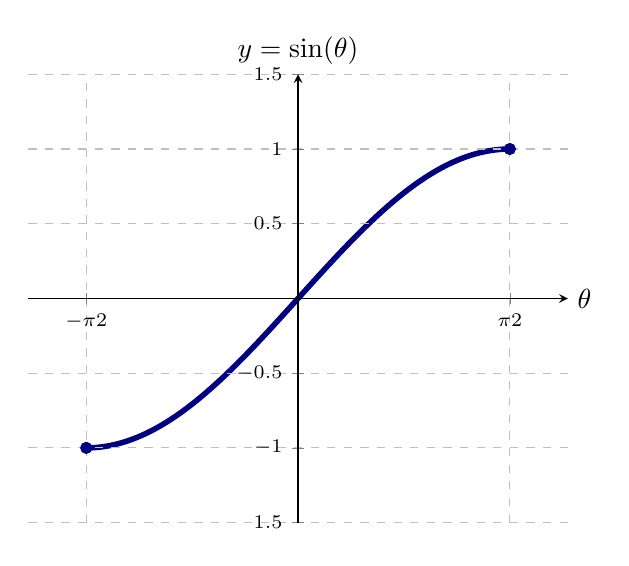
\begin{tikzpicture}
  \begin{axis}[
            domain=-2:2, ymax=1.5, xmax=2, ymin=-1.5, xmin=-2,
            axis lines =center, xlabel={$\theta$}, ylabel={$y = \sin(\theta)$}, grid = major, grid style={dashed},
            ytick={-1.5,-1,-0.5,0.5,1,1.5},
            xtick={-1.57, 1.57},
            xticklabels={$-\tfrac{\pi}{2}$, $\tfrac{\pi}{2}$},
            yticklabels={$1.5$,$-1$,$-0.5$,$0.5$,$1$,$1.5$}, 
            ticklabel style={font=\scriptsize},
            every axis y label/.style={at=(current axis.above origin),anchor=south},
            every axis x label/.style={at=(current axis.right of origin),anchor=west},
            axis on top
          ]
          

            \addplot [line width=2, penColor, smooth,samples=300,domain=(-1.57:1.57)] {sin(deg(x)};
            \addplot[color=penColor,fill=penColor,only marks,mark=*] coordinates{(-1.57,-1)};
            \addplot[color=penColor,fill=penColor,only marks,mark=*] coordinates{(1.57,1)};
            %\addplot [line width=2, penColor2, smooth,samples=300,domain=(-10:10),<->] {cos(deg(x)};



  \end{axis}
\end{tikzpicture}
\end{image}



It is only half a period, but it does cover the whole range of sine. And, more importantly, it covers every funciton value exactly once.

We can now reverse all of the pairs and obtain the inverse function known as \textbf{arcsine}.









\begin{image}
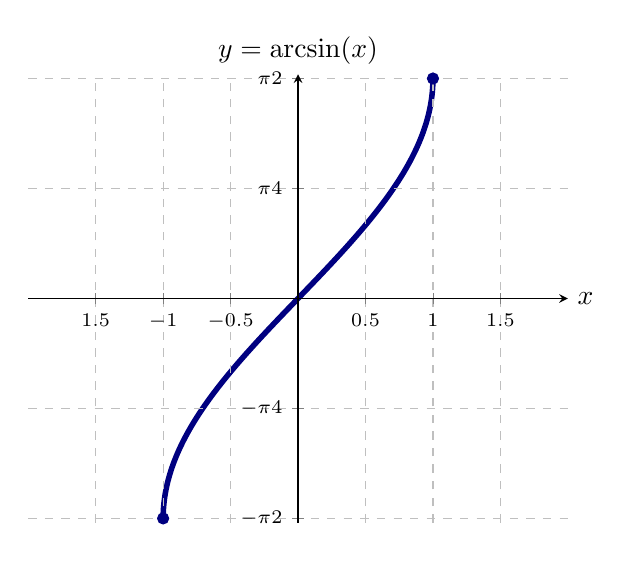
\begin{tikzpicture}
  \begin{axis}[
            domain=-2:2, ymax=1.6, xmax=2, ymin=-1.6, xmin=-2,
            axis lines =center, xlabel={$x$}, ylabel={$y = \arcsin(x)$}, grid = major, grid style={dashed},
            xtick={-1.5,-1,-0.5,0.5,1,1.5},
            ytick={-1.57,-0.785,0.785,1.57},
            yticklabels={$-\tfrac{\pi}{2}$, $-\tfrac{\pi}{4}$, $\tfrac{\pi}{4}$, $\tfrac{\pi}{2}$},
            xticklabels={$1.5$,$-1$,$-0.5$,$0.5$,$1$,$1.5$}, 
            ticklabel style={font=\scriptsize},
            every axis y label/.style={at=(current axis.above origin),anchor=south},
            every axis x label/.style={at=(current axis.right of origin),anchor=west},
            axis on top
          ]
          

            \addplot [line width=2, penColor, smooth,samples=300,domain=(-1.57:1.57)] ({sin(deg(x)},{x});
            \addplot[color=penColor,fill=penColor,only marks,mark=*] coordinates{(-1,-1.57)};
            \addplot[color=penColor,fill=penColor,only marks,mark=*] coordinates{(1,1.57)};
            %\addplot [line width=2, penColor2, smooth,samples=300,domain=(-10:10),<->] {cos(deg(x)};



  \end{axis}
\end{tikzpicture}
\end{image}




$Arcsine$ only returns angles between $-\frac{\pi}{2}$ and $\frac{\pi}{2}$. These are in the fourth and first quadrants. Arcsine is an inverse function for sine for these angles.



\begin{example}



$\sin\left(\frac{\pi}{6}\right) = \frac{1}{2}$

$\arcsin\left(\frac{1}{2}\right) = \frac{\pi}{6}$


$\arcsin\left(\sin\left(\frac{\pi}{6}\right)\right) = \frac{\pi}{6}$


\end{example}




When angles are outside $\left[-\frac{\pi}{2},\frac{\pi}{2}\right]$, then the Arcsine brings them back into this interval.




\begin{example}



$\sin\left(\frac{5\pi}{6}\right) = \frac{1}{2}$

$\arcsin\left(\frac{1}{2}\right) = \frac{\pi}{6}$


$\arcsin\left(\sin\left(\frac{5\pi}{6}\right)\right) = \frac{\pi}{6}$




We begin with the angle $\frac{5\pi}{6}$ whose sine is $\frac{1}{2}$.  Then Arcsine looks for an angle whose sine is $\frac{1}{2}$.  But Arcsine only looks in quadrants I and IV.  So, it finds $\frac{\pi}{6}$.


\end{example}









\subsection*{Characteristics} 

We can deduce many characteristics about arcsine from sine.


$\blacktriangleright$ The domain is  $[-1, 1]$.


$\blacktriangleright$ The range is $\left[ -\frac{\pi}{2}, \frac{\pi}{2} \right]$


$\blacktriangleright$ Arcsine has one zero and that is $0$.


$\blacktriangleright$ Arcsine is an increasing function.

$\blacktriangleright$ Arcsine is a continuous function.

$\blacktriangleright$ Arcsine has a maximum of $\frac{\pi}{2}$, which occurs at $1$.

$\blacktriangleright$ Arcsine has a minimum of $-\frac{\pi}{2}$, which occurs at $-1$.



\begin{question}


If $0 < \theta < \frac{\pi}{2}$, then $\arcsin(\sin(\theta))$ is in quadrant

\begin{multipleChoice}
\choice[correct] {I}
\choice {II}
\choice {III}
\choice {IV}
\end{multipleChoice}

\end{question}






\begin{question}


If $\frac{\pi}{2} < \theta < \pi$, then $\arcsin(\sin(\theta))$ is in quadrant

\begin{multipleChoice}
\choice[correct] {I}
\choice {II}
\choice {III}
\choice {IV}
\end{multipleChoice}

\end{question}









\begin{question}


If $\pi < \theta < \frac{3\pi}{2}$, then $\arcsin(\sin(\theta))$ is in quadrant

\begin{multipleChoice}
\choice {I}
\choice {II}
\choice {III}
\choice[correct] {IV}
\end{multipleChoice}

\end{question}







\begin{question}


If $\frac{3\pi}{2} < \theta < 2\pi$, then $\arcsin(\sin(\theta))$ is in quadrant

\begin{multipleChoice}
\choice {I}
\choice {II}
\choice {III}
\choice[correct] {IV}
\end{multipleChoice}

\end{question}


















\begin{question}


If $0 < \theta < \frac{\pi}{2}$, then $\arcsin(\sin(\theta))$ equals

\begin{multipleChoice}
\choice[correct] {$\theta$}
\choice {$\pi - \theta$}
\choice {$\pi + \theta$}
\choice {$\theta - 2\pi$}
\end{multipleChoice}

\end{question}







\begin{question}


If $\frac{\pi}{2} < \theta < \pi$, then $\arcsin(\sin(\theta))$ equals

\begin{multipleChoice}
\choice {$\theta$}
\choice[correct] {$\pi - \theta$}
\choice {$\pi + \theta$}
\choice {$\theta - 2\pi$}
\end{multipleChoice}

\end{question}






\begin{question}


If $\pi < \theta < \frac{3\pi}{2}$, then $\arcsin(\sin(\theta))$ equals

\begin{multipleChoice}
\choice {$\theta$}
\choice[correct] {$\pi - \theta$}
\choice {$\pi + \theta$}
\choice {$\theta - 2\pi$}
\end{multipleChoice}

\end{question}






\begin{question}


If $\frac{3\pi}{2} < \theta < 2\pi$, then $\arcsin(\sin(\theta))$ equals

\begin{multipleChoice}
\choice {$\theta$}
\choice {$\pi - \theta$}
\choice {$\pi + \theta$}
\choice[correct] {$\theta - 2\pi$}
\end{multipleChoice}

\end{question}


























\section*{Arccosine}











The cosine function is not one-to-one.









\begin{image}
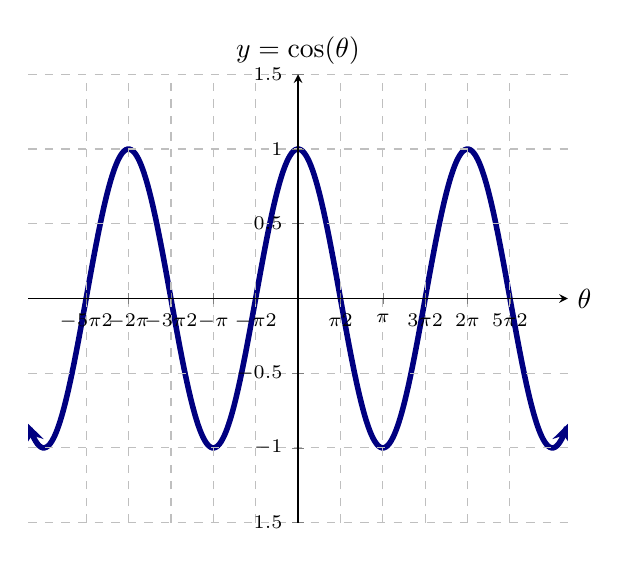
\begin{tikzpicture}
  \begin{axis}[
            domain=-10:10, ymax=1.5, xmax=10, ymin=-1.5, xmin=-10,
            axis lines =center, xlabel={$\theta$}, ylabel={$y = \cos(\theta)$}, grid = major, grid style={dashed},
            ytick={-1.5,-1,-0.5,0.5,1,1.5},
            xtick={-7.85, -6.28, -4.71, -3.14, -1.57, 0, 1.57, 3.142, 4.71, 6.28, 7.85},
            xticklabels={$-\tfrac{5\pi}{2}$,$-2\pi$,$-\tfrac{3\pi}{2}$,$-\pi$, $-\tfrac{\pi}{2}$, $0$, $\tfrac{\pi}{2}$, $\pi$, $\tfrac{3\pi}{2}$, $2\pi$, $\tfrac{5\pi}{2}$},
            yticklabels={$1.5$,$-1$,$-0.5$,$0.5$,$1$,$1.5$}, 
            ticklabel style={font=\scriptsize},
            every axis y label/.style={at=(current axis.above origin),anchor=south},
            every axis x label/.style={at=(current axis.right of origin),anchor=west},
            axis on top
          ]
          

            \addplot [line width=2, penColor, smooth,samples=300,domain=(-10:10),<->] {cos(deg(x)};
            %\addplot [line width=2, penColor2, smooth,samples=300,domain=(-10:10),<->] {cos(deg(x)};



  \end{axis}
\end{tikzpicture}
\end{image}





This function doesn't have an inverse.

We can't even restrict our domain to one period, because of the hills and valleys in the graph.

Therefore, our plan is to restrict the domain to half of one period of cosine.  We need a strategic interval of length $\pi$.  The usual choice is $[0,\pi]$.  














\begin{image}
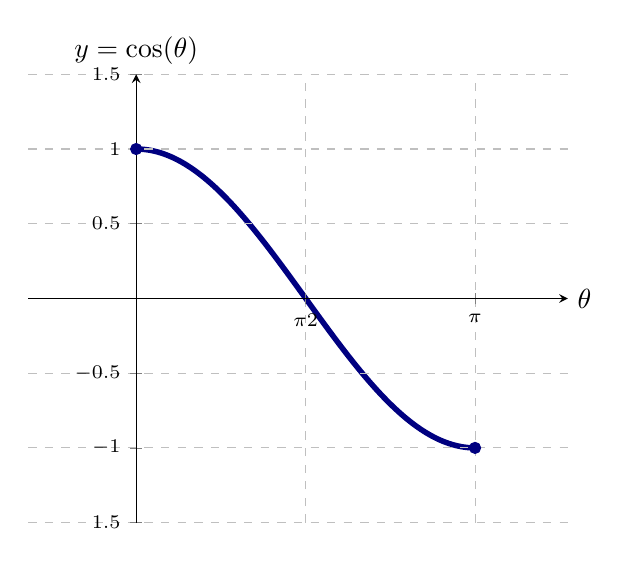
\begin{tikzpicture}
  \begin{axis}[
            domain=-1:4, ymax=1.5, xmax=4, ymin=-1.5, xmin=-1,
            axis lines =center, xlabel={$\theta$}, ylabel={$y = \cos(\theta)$}, grid = major, grid style={dashed},
            ytick={-1.5,-1,-0.5,0.5,1,1.5},
            xtick={1.57,3.14},
            xticklabels={$\tfrac{\pi}{2}$, $\pi$},
            yticklabels={$1.5$,$-1$,$-0.5$,$0.5$,$1$,$1.5$}, 
            ticklabel style={font=\scriptsize},
            every axis y label/.style={at=(current axis.above origin),anchor=south},
            every axis x label/.style={at=(current axis.right of origin),anchor=west},
            axis on top
          ]
          

            \addplot [line width=2, penColor, smooth,samples=300,domain=(0:3.14)] {cos(deg(x)};
            \addplot[color=penColor,fill=penColor,only marks,mark=*] coordinates{(0,1)};
            \addplot[color=penColor,fill=penColor,only marks,mark=*] coordinates{(3.14,-1)};
            %\addplot [line width=2, penColor2, smooth,samples=300,domain=(-10:10),<->] {cos(deg(x)};



  \end{axis}
\end{tikzpicture}
\end{image}



It is only half a period, but it does cover the whole range of cosine.

We can now reverse all of the pairs and obtain the inverse function known as \textbf{arccosine}.










\begin{image}
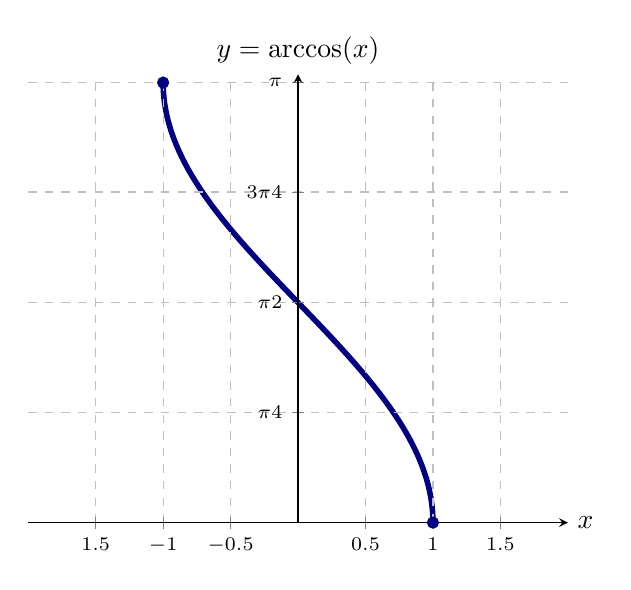
\begin{tikzpicture}
  \begin{axis}[
            domain=-2:2, ymax=3.2, xmax=2, ymin=0, xmin=-2,
            axis lines =center, xlabel={$x$}, ylabel={$y = \arccos(x)$}, grid = major, grid style={dashed},
            xtick={-1.5,-1,-0.5,0.5,1,1.5},
            ytick={0.785,1.57,2.36,3.14},
            yticklabels={$\tfrac{\pi}{4}$, $\tfrac{\pi}{2}$, $\tfrac{3\pi}{4}$, $\pi$},
            xticklabels={$1.5$,$-1$,$-0.5$,$0.5$,$1$,$1.5$}, 
            ticklabel style={font=\scriptsize},
            every axis y label/.style={at=(current axis.above origin),anchor=south},
            every axis x label/.style={at=(current axis.right of origin),anchor=west},
            axis on top
          ]
          

            \addplot [line width=2, penColor, smooth,samples=300,domain=(0:3.141)] ({cos(deg(x)},{x});
            \addplot[color=penColor,fill=penColor,only marks,mark=*] coordinates{(-1,3.141)};
            \addplot[color=penColor,fill=penColor,only marks,mark=*] coordinates{(1,0)};
            %\addplot [line width=2, penColor2, smooth,samples=300,domain=(-10:10),<->] {cos(deg(x)};



  \end{axis}
\end{tikzpicture}
\end{image}









$Arccosine$ only returns angles between $0$ and $\pi$.  It is an inverse function for these angles.





\begin{example}



$\cos\left(\frac{2\pi}{3}\right) = -\frac{1}{2}$

$\arccos\left(-\frac{1}{2}\right) = \frac{2\pi}{3}$


$\arccos\left( \cos\left( \frac{2\pi}{3} \right) \right) = \frac{2\pi}{3}$


\end{example}




When angles are outside $\left[ 0,\pi \right]$, then the Arcsine brings them back into this interval.




\begin{example}



$\cos\left(\frac{7\pi}{6}\right) = -\frac{\sqrt{3}}{2}$

$\arccos\left(\frac{-\sqrt{3}}{2}\right) = \frac{5\pi}{6}$


$\arccos\left(\cos\left(\frac{7\pi}{6}\right)\right) = \frac{5\pi}{6}$




We begin with the angle $\frac{5\pi}{6}$ whose cosine is $-\frac{\sqrt{3}}{2}$.  Then Arccosine looks for an angle whose cosine is $-\frac{\sqrt{3}}{2}$.  But Arccosine only looks in quadrants I and II.  So, it finds $\frac{5\pi}{6}$.


\end{example}











\subsection*{Characteristics} 

We can deduce many characteristics about arccosine from cosine.


$\blacktriangleright$ The domain is  $[-1, 1]$.


$\blacktriangleright$ The range is $[0, \pi]$


$\blacktriangleright$ Arccosine has one zero and that is $1$.


$\blacktriangleright$ Arccosine is an decreasing function.

$\blacktriangleright$ Arccosine is a continuous function.

$\blacktriangleright$ Arccosine has a maximum of $\pi$, which occurs at $-1$.

$\blacktriangleright$ Arccosine has a minimum of $0$, which occurs at $1$.








\begin{question}


If $0 < \theta < \frac{\pi}{2}$, then $\arccos(\cos(\theta))$ is in quadrant

\begin{multipleChoice}
\choice[correct] {I}
\choice {II}
\choice {III}
\choice {IV}
\end{multipleChoice}

\end{question}






\begin{question}


If $\frac{\pi}{2} < \theta < \pi$, then $\arccos(\cos(\theta))$ is in quadrant

\begin{multipleChoice}
\choice {I}
\choice[correct] {II}
\choice {III}
\choice {IV}
\end{multipleChoice}

\end{question}









\begin{question}


If $\pi < \theta < \frac{3\pi}{2}$, then $\arccos(\cos(\theta))$ is in quadrant

\begin{multipleChoice}
\choice {I}
\choice[correct] {II}
\choice {III}
\choice {IV}
\end{multipleChoice}

\end{question}







\begin{question}


If $\frac{3\pi}{2} < \theta < 2\pi$, then $\arccos(\cos(\theta))$ is in quadrant

\begin{multipleChoice}
\choice[correct] {I}
\choice {II}
\choice {III}
\choice {IV}
\end{multipleChoice}

\end{question}


















\begin{question}


If $0 < \theta < \frac{\pi}{2}$, then $\arccos(\cos(\theta))$ equals

\begin{multipleChoice}
\choice[correct] {$\theta$}
\choice {$\pi - \theta$}
\choice {$\pi + \theta$}
\choice {$2\pi - \theta$}
\end{multipleChoice}

\end{question}







\begin{question}


If $\frac{\pi}{2} < \theta < \pi$, then $\arccos(\cos(\theta))$ equals

\begin{multipleChoice}
\choice[correct] {$\theta$}
\choice {$\pi - \theta$}
\choice {$\pi + \theta$}
\choice {$2\pi - \theta$}
\end{multipleChoice}

\end{question}






\begin{question}


If $\pi < \theta < \frac{3\pi}{2}$, then $\arccos(\cos(\theta))$ equals

\begin{multipleChoice}
\choice {$\theta$}
\choice {$\pi - \theta$}
\choice {$\pi + \theta$}
\choice[correct] {$2\pi - \theta$}
\end{multipleChoice}

\end{question}






\begin{question}


If $\frac{3\pi}{2} < \theta < 2\pi$, then $\arccos(\cos(\theta))$ equals

\begin{multipleChoice}
\choice {$\theta$}
\choice {$\pi - \theta$}
\choice {$\pi + \theta$}
\choice[correct] {$2\pi - \theta$}
\end{multipleChoice}

\end{question}










\begin{center}
\textbf{\textcolor{green!50!black}{ooooo-=-=-=-ooOoo-=-=-=-ooooo}} \\

more examples can be found by following this link\\ \link[More Examples of Inverse Trig Functions]{https://ximera.osu.edu/csccmathematics/precalculus2/precalculus2/inverseTrigFunctions/examples/exampleList}

\end{center}





\end{document}
